% Yes, basically, your disks are big and dense.  But again, the organization of this section needs work.  Here are some suggestions:

% - Start off comparing basic stuff like masses and radii of your disks, so that we get the idea that relative to large populations of disks they are big and dense, but that relative to Sam’s disk they are comparable in mass/radius.

% - Then, delve into the chemistry.  You might consider starting by describing the models, so that we know what to expect.  Talk about what the models predict, then talk about how your disks fit in with those predictions.  Then bring in the other observation’s: you can do a pretty detailed comparison of your disk vs. Sam’s disk (in the table, yes, but also discussed in words in the text) and then you can compare with disks from low-mass SF regions as well (again, you’ve got a lot of the seeds of that discussion here).

% - The thing that’s really missing from the discussion is a conversation about what this all means.  *Why* might the similarities/differences between your disk and Sam’s, or your disk and the ones in low-mass SFRs exist?  I think you will be able to write it a lot better once you have expanded your reading beyond just Catherine Walsh’s modeling.  What factors do the modelers predict should affect the chemistry of these disks?  How are these factors related to environment?  To what extent might they be influenced by binarity?  


\chapter{Discussion}
\label{chap:discussion}

With the disks now fit, we may interpret our results. Since this project was based around the question of how environment influences protoplanetary disks, we would like to compare our best fit values to other disks, including to one other from the ONC \citep{Factor2017} as well as to others outside of it. We also consider how our results compare to modeling efforts.


\section{Reflections on the Fits}

As discussed in \S\ref{subsection:co_fit}, our attempts to fit the CO line were overwhelmed by the significant cloud contamination around the disk, resulting in physically-unreasonable best-fit values. If this run had converged to physical values, we would have used its disk mass results in the other runs, but since these results are not to be trusted, we instead continued to use the disks' mass values presented in \citet{Williams2014}, which were inferred from continuum emission.


% I think you should be specific about what “high chemical abundances” means here.  Which molecules are more abundant than expected, and relative to what?  (Models?  Other disks?)  

The \hco and HCN runs converged into impressive agreement, although the posteriors from the \hco line show smaller uncertainties than those of the HCN line. Both the \hco and HCN lines show surprisingly high abundances in disk A, while both also show significantly lower values for disk B abundances (discussed below). The two lines' fits for disk A's outer radius agree to within around 1\% (although the HCN fit is significantly less certain than the \hco fit) and the lines' best-fit $q$ values agree to within 15\%. Atmospheric temperatures for disk A in both lines are large and significantly different, with the \hco line preferring a temperature 50\% greater than HCN's, but this is at least somewhat expected, as the two molecules are emitting from different regions of the disk and thus could reflect different regions of its temperature profile. In both lines, disk A's temperature structure power law index, $q$, is decidedly positive, although we expect this parameter to not settle with absolute certainty on a single value, since the observations don't have enough spatial resolution to constrain it tightly.
% REWORK: be quantitative about "decidedly"

% REWORK all percentages: I’m not really interested in what percentage agreement is reached, but rather the significance of that agreement.  Do they agree to within 1-sigma, for example?  All of these percentage values need to be rewritten in terms of significance.

% The 50% figure is a little more interesting, but here I might just insert the actual values.  Something like: “The best-fit atmospheric temperature for HCO+ (xxx+/-xxx K) is significantly higher/lower than the corresponding value for HCN (xxx+/-xxx K), but this is at least somewhat expected…”


% REWORK: does this "as discussed previously" make sense?
% REWORK: Reference to "connecting feature" is explained two pars down - straighten this out.
% REWORK: This whole paragraph is garbage.
% REWORK: What does expected mean? Useful?
Fits for disk B are systematically less well constrained, since it is smaller, unresolved, and more easily overrun by emission from features that were not modeled, such as cloud contamination, excess disk A emission, and the connecting feature between the disks. As discussed previously, the outer radius was most notably affected by these features, as it yielded somewhat bimodal posteriors in both lines REWORK IS THIS TRUE CHECK CORNERs as the walkers sometimes tried to fit the outer features. Still, save for the disk's outer radius fit, all parameters are generally within the range of expected values.



As discussed in \S\ref{subsection:hcn_fit}, a posteriori cuts of the HCN model's MCMC chain limiting disk B's outer radius to $\geq$220 AU changes the best-fit parameters significantly, most notably leading the fits of disk B's outer radius in \hco and HCN into agreement and pushing disk A's HCN abundance more than a full order of magnitude higher, and into nearly perfect agreement with results from HCN fitting in \citet{Factor2017}. Whether this is a reasonable thing to do is not clear to me.

We see in the HCN channel maps an area of significant flux coming from between disks around $ v = 11-9$ \kms. This may be region where the two disks are interacting, a possibility that our model does not take into account. The feature is less clearly present in \hco and invisible in CO, likely overrun by cloud contamination.


% REWORK: "Yes, very speculative.  How about mentioning some other possibilities?  For example, if the central stars are different spectral types, that could affect the photochemistry, or different initial disk masses/optical depths could affect how the disks evolve, or planets… try thinking of some more possibilities, and dig into the literature to find some references (they are out there!)""
That each disk's abundances are so different from one another is something of a surprise. Both disks have fairly similar ratios of the two emitting molecules: disk A's \hco/HCN ratio of log abundances is 1.09, while disk B's is 0.95\footnote{These ratios become 1.21 for disk A and unity for disk B if the disk B radius cut is made.}. \citet{Williams2014} posit that wide binaries (systems with separations $\geq$ 300 au), such as this one, do not form in the same initial cloud structures\footnote{Jonathan doesn't actually put any references on this; I have no idea where he got it from. He just puts in references to other papers looking at misaligned binaries}. If this is the case, the notable differences in abundances between disk A and disk B could indicate that the disks in d253-1536 formed separately in clouds with different chemical compositions before joining together later. This is, of course, entirely speculative, but is a possibility.
% REWORK: Re the footnote: "Hm, I’m not sure either, but I would take a look at Robert Harris’s PhD thesis papers on binaries with the SMA as a starting point — check his intro and discussion for relevant references.  Could also check the more recent Akeson/Jensen papers on binaries with ALMA for some relevant intro/discussion material.  Would be good to expand upon this point in the discussion."




\section{Comparison with the Literature}
% REWORK: How this whole chapter is organized.

\subsection{Line Emission Modeling}

% REWORK: See if this table prints better (no RHS cutoff) without \centering
% REWORK: "In terms of content, this is a great start, but how exhaustive is it?  I think you need to specify exactly what you’re doing with this table, and how you decided which disks to compare with and which ones not to.  The French group (Guilloteau, Dutrey, and others) would be very upset that you didn’t include any of their work, for example!  I really like the idea behind this table, but I think you need to go big or go home — make sure you’re specific about what is included in the table, and then make sure you are thorough about including all the relevant studies."
\begin{table}[ht!]
  % \centering
  \begin{threeparttable}
    \caption{Disk Parameter List}
    \label{table:comparisons}
    \renewcommand{\arraystretch}{1.2}
    \begin{tabular}{l l l c c c }
      \toprule \toprule
      %\multirow{2}{*}{Parameter} & \multirow{2}{*}{Disk A}    & \multicolumn{2}{c}{Disk B} \\
      Reference                             & Source     & Line          & $q$ & log X$_\text{mol}$ & Atms. Temp\\
      \midrule %\midrule
      \multirow{3}{*}{This study}           & d253-1536a & \hco(4-3)      & $0.66$  & $-7.96$         & $151$  \\
                                            & d253-1536a & HCN(4-3)       & $0.72$  & $-7.62$         & 140  \\
                                            & d253-1536a & CO(3-2)\tnote{a} & $0.40$  & $[-4]$        & 1  \\
      \hline
      \multirow{3}{*}{\cite{Factor2017}}   & d216-0939  & \hco(4-3)      & $0.17$  & $-10.08$        & 190  \\
                                           & d216-0939  & CO(3-2)        & $-0.33$ & $[-4]$          & 70  \\
                                           & d216-0939  & HCN(4-3)       & $-0.18$ & $-6.7$          & 19  \\
      \hline
      \multirow{2}{*}{\citet{Flaherty2015}}& HD163296   & CO(3-2)        & $-0.22$ & $[-4]$          & 94  \\
                                           & HD163296   & CO(2-1)        & $-0.27$ & $[-4]$          & 79  \\
      \hline
      \citet{Hughes2008}\tnote{b}           & A bunch    & CO(3-2)        &  -    & $[-4]$          & -  \\
      \hline
      \citet{Rosenfeld2012}\tnote{b}        & V4046 Sgr  & $^{12}$CO(2-1) & $-0.63$ & $[-4]$           & -  \\
      \hline
      \citet{Flaherty2017}\tnote{c}         & HD163296   & DCO$^+$(3-2)   & $[-2.22]$ & $-10.79$      & [94]  \\
      \hline
      \citet{Zhang2017}                     & TW Hya     & $^{13}$C$^{18}$O(3-2), C$^{18}$O(3-2)  & $-0.47$ & -7.96 & 151  \\
      \hline
      \citet{Flaherty2018}\tnote{d}         & TW Hya     & CO(6-5, 3-2, 2-1) & $-0.46$ & $[-4]$       & 31  \\
      \bottomrule
    \end{tabular}
    \begin{tablenotes}\footnotesize
      \item[*] Values in [brackets] were fixed during fitting.
      \item[\dagger] Since there is not a convention about whether a negative value of $q$ indicates a radially decreasing or increasing temperature structure (in other words, whether or not $q$ is implicitly negative), some of these values have the opposite sign of the value reported in their article. When this is the case, it indicates that, in that original paper, atmospheric temperature was defined such that T$_{atms} \propto r^{-q}$. In our work, and in all the values given here, it is the case that T$_{atms} \propto r^{q}$, meaning that a negative value of $q$ leads to temperature decreasing with radius.
      \item[a] This result is being presented for completeness (and to allow for the chance that something changes dramatically in coming runs REWORK), but since its T$_{atms}$ clearly got stuck, it is not a useful result for comparison and will not be discussed.
      \item[b] \cite{Rosenfeld2012} didn't fit for tatms
      \item[c] In \citet{Flaherty2017}, they fit three rings, and consequently have three slightly different values for each parameter. The values reported here are for their middle ring, although the three do not vary significantly from one another. Additionally, T$_{atms}$ and $q$ were fixed at values found for CO(3-2) in \citet{Flaherty2015}, and only X$_\text{mol}$ was fit for.
      \item[d] \citet{Flaherty2018} developed several models, with different morphological structures. The results presented here are drawn from their simplest (fiducial) model.
    \end{tablenotes}
  \end{threeparttable}
\end{table}




Our molecular abundances for each disk vary from those reported in the \citet{Factor2017} paper, the only other study to do forward-modeling of \hco emission using a ray tracing code. In it, they report finding canonical values for the \hco line (log X$_{\text{HCO}^+}$ = $-10.04$) and unexpectedly high values for the HCN line (log X$_{HCN}$ = $-6.7$), contrasted by our findings of $-8.36$ and $-7.62$, respectively\footnote{Although, as described above, removing samples with large outer radii for disk B pushes disk A's HCN abundance to -6.98, within the uncertainties of their HCN fit.}.


% REWORK: I think somewhere before this section, ideally right at the start of the chapter, you should lay out a bunch of caveats about our abundances — particularly that they are derived from the MAJOR assumption the total disk gas mass will be 100x the dust mass derived from continuum emission.  It needs to be in everyone’s mind while they are reading about the modeling.  
We may also compare these abundances to theoretical modeling efforts. \citet{Walsh2010} developed radial and vertical chemical models for an isolated protoplanetary disk around a T-Tauri star (a system with physical parameters similar to the famous TW Hya and its disk), studying molecular abundance distributions throughout the disk for molecules within ALMA's reach. They showed that log abundances in their models for \hco varied from $-8$ to $-12$, $-7$ to $-12$ for HCN, and $-4$ to $-9$ for CO. The authors then built on this model by adding robust modeling of externally-driven UV and X-ray ionization \citep{Walsh2012} and applying it to the same disk system, this time with an O star nearby providing ionizing photons \citep{Walsh2013}. They then make the same molecular abundance distribution maps as before (see Fig. \ref{fig:walsh-abundance-profs}). The authors note that, in their model photoionized disk, \hco column density increases by a factor of 6.3 relative to the isolated disk, whereas HCN and CO column densities remain constant through ionization\footnote{This would be useful if we had an estimation of what the \hco/HCN ratio would be in these two disks. They do have column density ratios in Walsh13; is it reasonable to say (I guess it would have to be in the case of optically thin emission) that col dens $\propto$ abundance? If that were the case then we'd be golden.}. They also note that the ionized disks have much higher gas temperatures, $\gg$ 50 K, which is consistent with our findings.
% REWORK: There’s more to this field than one series of papers by Catherine Walsh!  Need to represent the whole diversity of the field.  Look up papers by Yuri Aikawa, Ted Bergin’s group, 


Although our modeling assumes a constant chemical abundance across the whole disk, these models offer a way to confirm that our results are within the predicted ranges, despite the fact that the \hco abundance is significantly higher than the values found by other studies.



\begin{figure}[t]
  \hspace*{\fill}%
  \subcaptionbox{CO abundances}{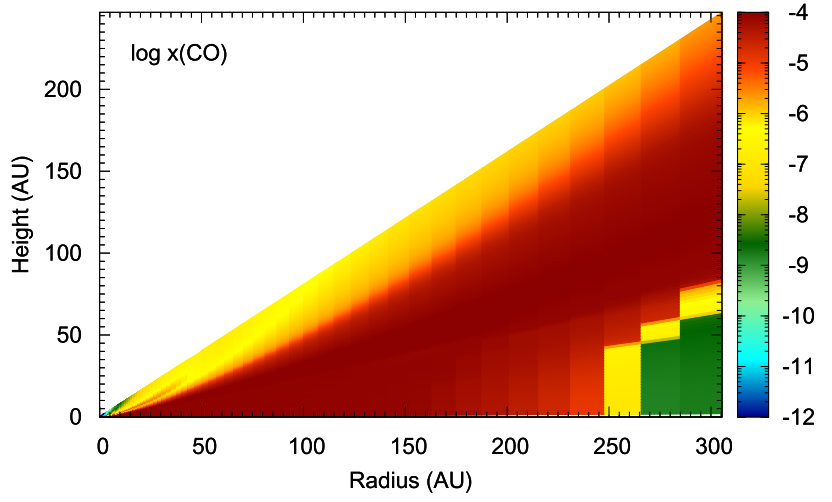
\includegraphics[width=0.33\linewidth]{walsh10_Xco.png}}%
  \subcaptionbox{\hco abundances}{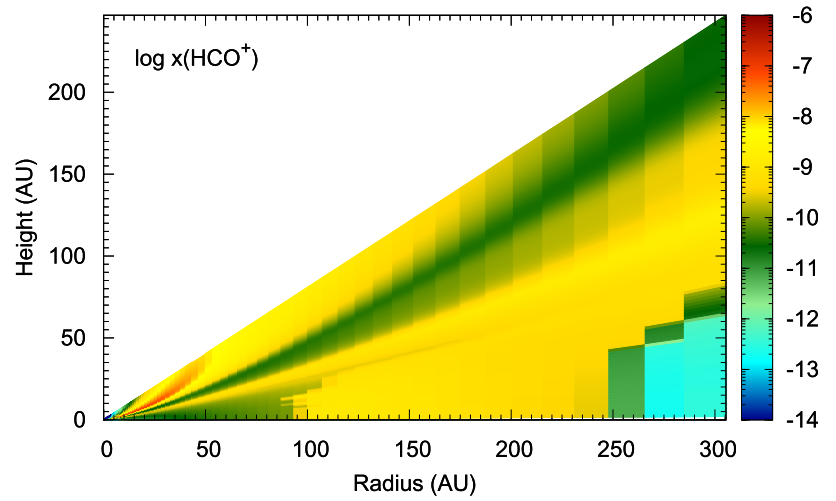
\includegraphics[width=0.33\linewidth]{walsh10_Xhco.png}}%
  \subcaptionbox{HCN abundances}{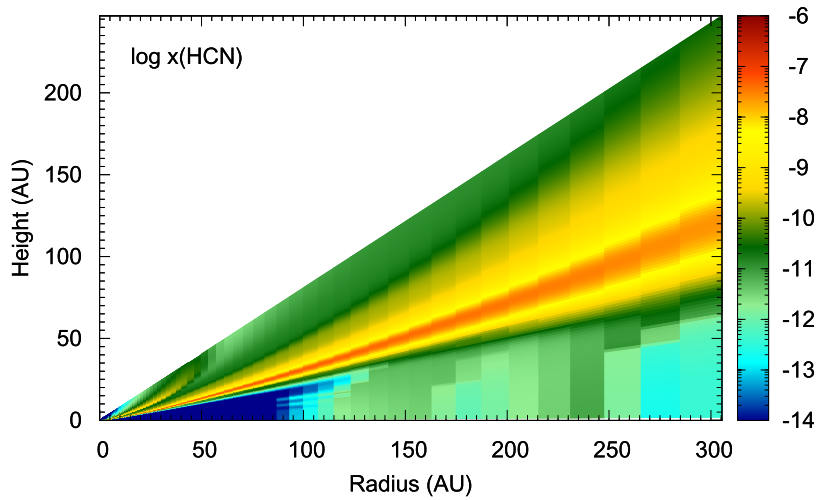
\includegraphics[width=0.33\linewidth]{walsh10_Xhcn.png}}\vfill%
  \subcaptionbox{CO abundances}{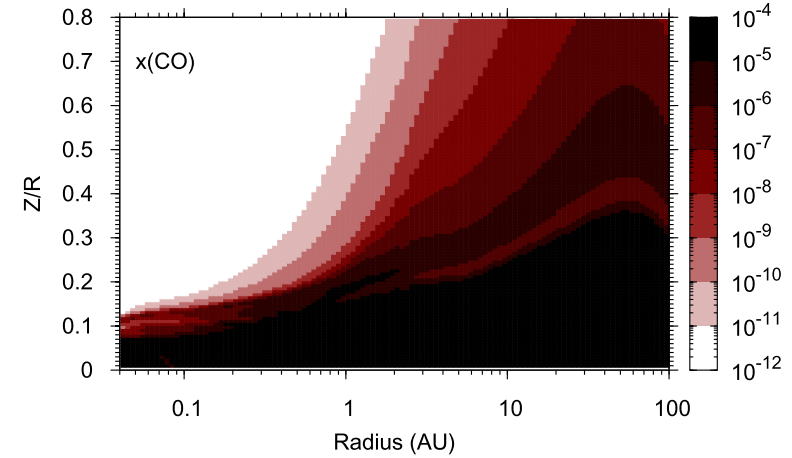
\includegraphics[width=0.33\linewidth]{walsh13_Xco.png}}%
  \subcaptionbox{\hco abundances}{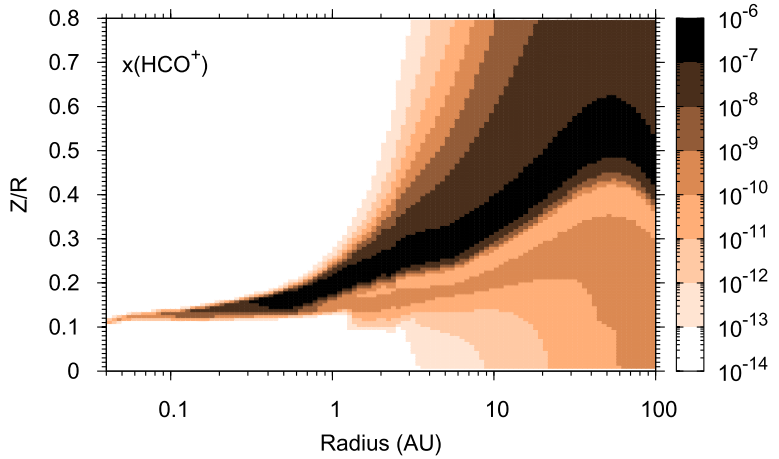
\includegraphics[width=0.33\linewidth]{walsh13_Xhco.png}}%
  \subcaptionbox{HCN abundances}{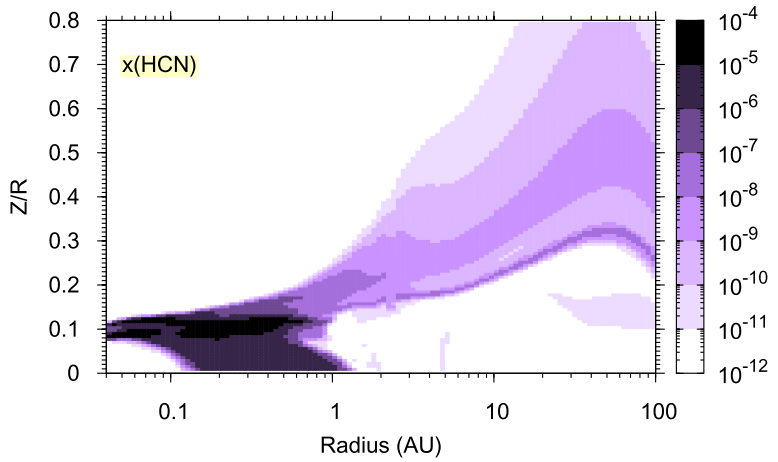
\includegraphics[width=0.33\linewidth]{walsh13_Xhcn.png}}%
  \hspace*{\fill}%
  \caption{Models showing radial and vertical distributions of CO, \hco, and HCN in a simulated disk around a T-Tauri star. The top row shows the profiles of isolated disks \citep{Walsh2010}, while the bottom row shows the profiles of disks being irradiated by a nearby O star \citep{Walsh2013}. Note that bottom row is on a log scale and only covers the inner 100 AU of the disk, while the top row is linearly scaled and shows a 300AU stretch. \textit{It seems like only having one of these sets of images would make more sense.}}
  \label{fig:walsh-abundance-profs}
\end{figure}




\subsection{Population Comparison}

We can also compare our disks' mass and radius to other protoplanetary disks. While these features may provide less nuanced insight, they are more easily measured, giving us a broader sample of disks to compare ours to. For these comparisons, we again draw on the disks' inferred gas mass measurements made by \citet{Williams2014}, which carry with them significant uncertainty on account of the 100:1 assumed gas:dust ratio (as described in \S\ref{chap:introduction}). As such, the values we use for the masses of disk A and disk B are 0.075 M$_\odot$ and 0.029 M$_\odot$ (78.66 and 29.88 Jovian masses), respectively. Our best-fit values for radii from the MCMC models were around 337 and 145 AU, respectively.


% REWORK: "“of the disks’ radial extents, [based on…]” (i.e., say how they estimated the radial extent, so that it is clear when you’re comparing apples to apples and when you’re not)."
% REWORK: Check that the first Factor2017 reference prints correctly using the trick citet syntax
In the survey that originally provided these data, \citet{Mann2014} calculated initial disk masses, as well as semi-minor and -major axes of the disks, approximate measures of the disks' radial extents. Disk A in the present system was, by their measure, the most massive disk in the study, 75\% more massive than the study's next most massive disk, d216-0939 \citet[which was the subject of][]{Factor2017}; disk B was the fifth most massive. Disk A had the study's fourth largest semi-major axis\footnote{The authors' measurement of disk A's semi-major axis, at 268 au, is 20\% smaller than our fit measurements. The survey's reported semi-major axis for d216-0939 was also smaller than the fit value in \citet{Factor2017}, though by only 6\%.}. The authors did not fit disk B's radial extent; however, our measurement of 145 AU would make it the eleventh (out of 22) largest disk in the survey. Thus, disk A is on the very high end of the study's mass and radius range, while disk B is apparently quite dense and of median radial extent.


% REWORK: Why lower-than-expected
% REWORK: I’m not sure this is the study you want to talk about here, or how you want to present it.  A couple of thoughts:
% - You start off comparing the disks’ masses and radii to other disks in Orion, which is great.  Clearly apples to apples.
% - Next, you want to compare your disks to disks in low-mass SF regions.  Also great.  But to discuss how the properties of your disks compare to the properties of disks in low-mass SF regions, you need to compare the same data.  So you’d want to look for a study (and there are lots! some of which you talk about below!) that compiled disk masses based on mm continuum measurements, assuming 100:1 gas:dust mass ratio like Rita did.
% - The study you’re referencing here is really great and important!  But I think you want to discuss it in the context of the assumptions you made and why they might not be correct.  Specifically, this study provides evidence that 100:1 may not be a valid assumption for the gas:dust mass ratio in protoplanetary disks.
% So, all good stuff, but just organized weirdly.  I think you should also describe a bit more of the methodology of how the authors “analyze several CO isotopologues” — this is a nonstandard (but very interesting!) method that involves comparison of data with radiative transfer models of a large grid of generic disk models, so you should say a bit more about what they did so that your reader can better interpret it.  
In \citet{Miotello2016}, the authors analyze several CO isotopologues to retrieve the gas masses of 34 protoplanetary disks in Lupus. In it, they report lower-than-expected masses, reflective of their calculated gas/dust ratios, which systematically fall well below the ISM value of 100. Their resulting gas masses are far smaller than those found by \cite{Mann2014} in the ONC; here, most of the survey's masses are between $10^{-5}$ to $10^{-3}$ M$_\odot$, with the most massive at 1.5 $\times 10^{-3}$ M$_\odot$ (1.6 Jovian masses). since the disks were not spatially resolved, radii were not measured.


% REWORK: One thing you need to make sure to include in any discussion of disk mass ranges is a discussion of sensitivity limitations.  Are there disks with masses less than 1 M_Jup?  Probably!  Are they detectable?  Nope.  Also, the sensitivity limits are lower for low-mass SF regions than for high-mass, simply because they’re closer, which is another important caveat that is currently missing from your discussion. 
\citet{Ansdell2016} and \citet{Ansdell2018} characterized the mass (both dust and gas) and radius distributions of protoplanetary disks in Lupus using CO isotopologues and continuum emission. To derive gas masses, they assumed a CO/H$_2$ ratio of $10^{-4}$ and then used the isotopologues' ratios to find total masses. Of these gas masses that they were able to constrain, they found disks to range from around 1-10 Jovian masses.


\citet{Eisner2018} conducted a particularly comprehensive survey of disks in $\sigma$ Ori, a young cluster in the ONC, north of M42 and M43. In their survey, they trace dust masses, so maybe it's not terribly useful. Still, they note that disks in their survey are particularly compact.
% REWORK (on "it's not terribly useful"): It is!  You can make the same 100:1 assumption as the other studies to compare the data.  This is a great study to include in the comparison, since it is also a high-mass region.


\begin{figure}[h!]
  \centering
    \hspace*{\fill}%
    \subcaptionbox{\hco}{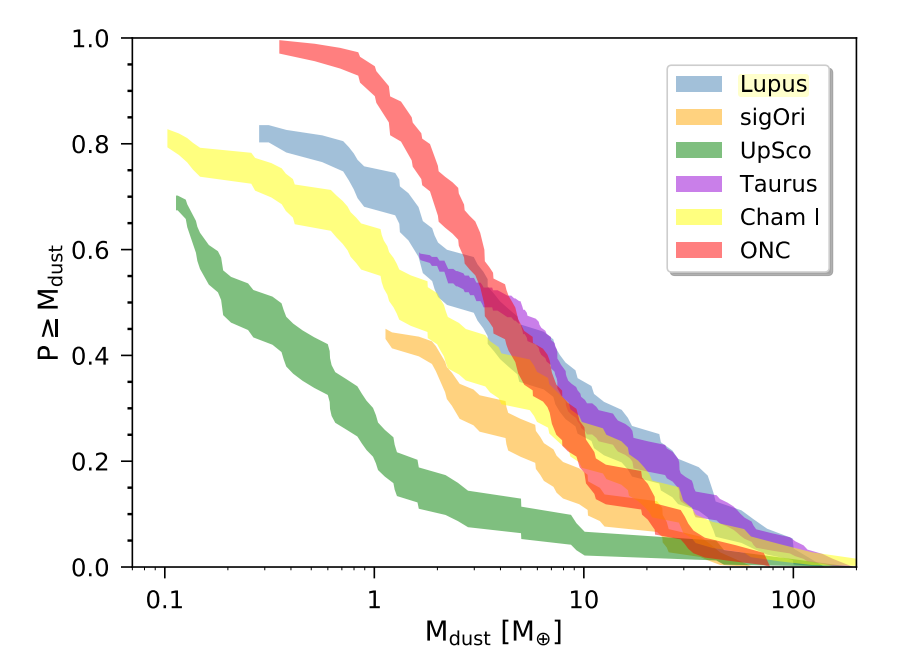
\includegraphics[width=0.5\linewidth]{dust_mass_dist_Eisner18.png}}%
    \subcaptionbox{HCN}{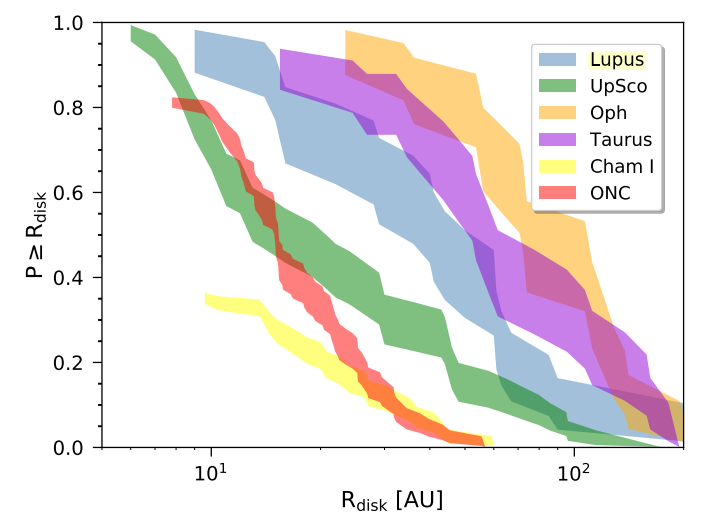
\includegraphics[width=0.5\linewidth]{dust_radius_dist_Eisner18.png}}%
    \hspace*{\fill}%
    \caption{Some stuff from Eisner2018.}
    \label{fig:bf_disk_strs}
\end{figure}
% REWORK: Some really great stuff from Eisner 2018!  Give it a full caption and a full discussion in the text!  This is a critical piece of data on the role of environment in determining disk mass and radius distributions!



% \citet{Cieza2019} also has stuff for this

I don't really know what else to say here. Seems like ours are big, dense disks. Would be really nice to calculate that gas mass on my own.




% Kamp overview:
% https://arxiv.org/pdf/1901.10862.pdf




% No density profile == No MMSN bs
% \section{Planet-Forming Potential}
% \label{section:fitting_procedure}
%
%
% One way to contextualize the results presented in \S\ref{chap:analysis} is through the lens of planet formation. This analysis traditionally begins with a comparison to the MMSN, which is the density profile that our own Solar System would have if all our planets had gas added to them until their composition matched that of the Sun, then each planet's mass was spread out in a ring along its orbital path (as discussed in \S\ref{chap:introduction}). Integrating this mass leaves us with $M_\text{MMSN} \approx 0.01 M_\odot$. It is worth reiterating that this is an extremely rough metric, build on several assumptions, and that it does not reflect \textit{minimum} mass of a planet forming potential, but rather an approximation of the mass it would take for a disk like ours to form.
%
% With the extremely large mass of $M = 0.36M_\odot$ that we measure in the CO line, it is needless to say that the disk's mass would not be its limiting factor in planet formation.











% The End
